%%%%%%%%%%%%%%%%%%%%%%%%%%%%%%%%%%%%%%%%%%%%%%%%%%%%%%%
% A template for Wiley article submissions.
% Developed by Overleaf. 
%
% Please note that whilst this template provides a 
% preview of the typeset manuscript for submission, it 
% will not necessarily be the final publication layout.
%
% Usage notes:
% The "blind" option will make anonymous all author, affiliation, correspondence and funding information.
% Use "num-refs" option for numerical citation and references style.
% Use "alpha-refs" option for author-year citation and references style.

\documentclass[alpha-refs]{wiley-article}
% \documentclass[blind,num-refs]{wiley-article}

% Add additional packages here if required
\usepackage{siunitx}
\usepackage{lineno}

% Update article type if known
\papertype{Original Article}
% Include section in journal if known, otherwise delete
%\paperfield{Journal Section}

\title{Field monitoring of Onion Maggot (\textit{Delia antiqua}) fly through improved trapping}

% List abbreviations here, if any. Please note that it is preferred that abbreviations be defined at the first instance they appear in the text, rather than creating an abbreviations list.
%\abbrevs{ABC, a black cat; DEF, doesn't ever fret; GHI, goes home immediately.}

% Include full author names and degrees, when required by the journal.
% Use the \authfn to add symbols for additional footnotes and present addresses, if any. Usually start with 1 for notes about author contributions; then continuing with 2 etc if any author has a different present address.
\author[1\authfn{1}]{Denis S. Willett}
\author[1\authfn{1}]{Camila C. Filgueiras}
\author[1]{Jan P. Nyrop}
\author[1]{Brian A. Nault}

\contrib[\authfn{1}]{Equally contributing authors.}

% Include full affiliation details for all authors
\affil[1]{Department of Entomology, Cornell AgriTech, Cornell University, Geneva, NY, 14456, USA}

\corraddress{Denis S. Willett, 15 Castle Creek Drive, Geneva, NY 14456}
\corremail{deniswillett@cornell.edu}


% Include the name of the author that should appear in the running header
\runningauthor{Willett et al.}

\begin{document}

\maketitle

\begin{abstract}
Onion maggot (\textit{Delia antiqua}) is an economically important pest of Allium crops in temperate regions throughout the world.  Management of this pest is necessary to achieve economic returns and depends on insecticide regimes and cultural management.  Future management strategies for \textit{D. antiqua} may rely upon effective monitoring of \textit{D. antiqua} populations, but traditional means of monitoring can be ineffective at catching sufficient numbers of \textit{D. antiqua} flies to accurately reflect population dynamics. We evaluated the effect of shape, size, color and chemical attractants on trap catch of field populations of adult \textit{D. antiqua} flies in upstate New York. White, large diameter, spherical traps in conjunction with Delia Lure attractant performed the best in attracting and catching \textit{D. antiqua} adults. These results suggest an improved means of attracting and capturing \textit{D. antiqua} populations which could be useful in monitoring efforts and development of attract and kill strategies for pest control. 

% Please include a maximum of seven keywords
\keywords{Onion Maggot, \textit{Delia antiqua}, attraction, sticky-trap, attract-and-kill, lure, onion management}
\end{abstract}

\linenumbers
\section{Introduction}

The onion maggot (\textit{Delia antiqua} Meigen) is an economically important pest of Allium crops worldwide.  Found primarily in temperate climates, \textit{D. antiqua} is well established in onion growing regions in the Americas, Europe and Asia where crop losses due to this pest can range from 50 to 100 percent on onions (\textit{Allium cepa} L.), garlic (\textit{Allium sativum} L.), scallions (\textit{Allium fistulosum} L.), and chives (\textit{Allium schoenoprasum} L.) if left unmanaged \citep{ellis1979factors,ning2017predicting,nault2007ecology, nault2006performance, nault2006onion}.  Intensive management of this pest has become a necessary component of effective onion production in many parts of the world and severe damage from this pest continues to occur in areas where Allium crops are grown without rotation or where populations resistant to insecticides have developed \citep{martinson1988dispersal, nault2006onion}.  

\textit{D. antiqua} is a primary pest in part due to its lifecycle.  It is multivoltine with three generations per year in the Northern United States \citep{eckenrode1975population, hoepting2004insecticide}.  Larvae feed on plant roots and allium bulbs causing the damage associated with this pest.  First-generation infestations are particularly devastating as early feeding by \textit{D. antiqua} larvae can kill seedlings \citep{nault2006onion, nault2006performance}.  In addition, damaged plants become more susceptible to infestation by subsequent generations and pathogens \citep{eckenrode1986impact,nault2006performance}.  Even if plants are not completely killed by \textit{D. antiqua} larvae, feeding damage often renders the bulbs unmarketable.  

Management of this pest has relied on prophylactic insecticide applications at planting \citep{nault2006performance}.  A variety of organophosphate and carbamate insecticides have been used and discontinued \citep{nault2006performance}.  Chlorpyrifos is commonly used as a drench treatment in combination with either cyromazine seed treatment (Trigard)  \citep{nault2006performance} or the seed treatment package containing thiamethoxam, spinosad and several fungicides (FarMore FI500).  Cultural practices such as crop rotation, removal of cull and volunteer onions from fields, and delayed planting are also effective management tactics  \citep{martinson1988dispersal, finch1985influence, nault2011delaying}.  

In situations where an insecticide application at planting is not desired for \textit{D. antiqua} control, reliance on monitoring \textit{D. antiqua} adult activity in the field can be important for deploying curative management tactics. Additionally, effective monitoring becomes even more important where \textit{D. antiqua} is a relatively recent introduction or in areas where producers are not sure they have a problem. 

Past efforts at monitoring and understanding \textit{D. antiqua} phenology have relied on three principal methods: sticky traps, water traps, and simulation.  Sticky traps and water traps have been used to varying degrees of success in North America and Europe but often suffer from limitations related to inefficiencies in counting \citep{thomingdeveloping,otto2000development}.  Trap catch of adult \textit{D. antiqua} flies can be low compared to field populations.  Additionally, the number of \textit{D. antiqua} caught compared to other insect collected in traps necessitates a great deal of time in evaluating trap catches.  Odor sources of attractants also have been added to traps in an effort to make them more attractive, but with limited success.  Simulation has relied on field data from traps, phenological studies in the lab, and climate information \citep{thomingdeveloping,otto2000development,ning2017predicting}.  Population simulations can prove useful at larger scales, but often lack extremely detailed location specific information necessary for producers to determine if they have a severe problem in a specific field.  

To further develop effective monitoring methodologies for the \textit{D. antiqua}, we evaluated a number of factors likely to influence attraction of adult \textit{D. antiqua} flies.  Previous work has suggested that color, shape, size, and chemistry all affect attraction of adult \textit{D. antiqua} \citep{harris1983color,harris1988host, thomingdeveloping, otto2000development}. We expanded on previous work in field trials over two years in upstate New York where a variety of novel trap designs with varying shape, size, color, and chemistry were evaluated to capture adult \textit{D. antiqua}.  

\section{Materials and Methods}

To improve trap catch and monitoring of adult \textit{D. antiqua} flies, iterations of sticky traps of various shape, size, and color were evaluated in 2005 and 2006 in upstate New York.  Additionally, after an improved shape, size, and color trap was developed, this trap was tested in conjunction with a Delia Lure (AgBio, Westminster, CO) attractant to evaluate potential improvement in trap catch.  

All shape, size, and color trials were conducted in commercial dry bulb onion fields on muck soil near Elba, NY in western upstate New York. Muck soils are high-organic matter soils formed from old lake beds.  Trials evaluating trap catch in conjunction with Delia Lure were evaluated both in Elba, NY and on muck soil near Potter, NY in central upstate New York.  All locations used in these studies are characterized by continuous onion production with no-rotation and consistently high \textit{D. antiqua} populations.  No modifications were done to commercial weed, disease, or pest management and spray programs (which closely followed recommended management \citep{reiners2019}), the primary target of which is \textit{Thrips tabaci}. This management did not affect \textit{D. antiqua} populations as spray timing and efficacy of products targeting thrips have minimal to no impact on \textit{D. antiqua} adults \citep{finch1986behavior}. 

\subsection{Field Trials}

For all field trials, numbers of male and female \textit{D. antiqua} flies were recorded weekly from traps beginning in late May and ending in late June. 

\paragraph{Shape Trial} To evaluate effect of trap shape on trap catch and monitoring of adult \textit{D. antiqua} flies, square, cube, short cylindrical, tall cylindrical, and spherical semi-gloss white shapes each with a surface area of 180 $cm^2$  were coated with Tanglefoot sticky material (The Scotts Company LLC, Maryville, OH) and placed along the long edge of an onion (\textit{Allium cepa} L.) field near Elba, NY. Traps were spaced 15.2 meters apart and arranged in a randomized control block design with five replications.   

\paragraph{Size Trial}
To evaluate the influence of trap size on trap catch and monitoring of adult \textit{D. antiqua} flies, white spherical sticky traps with diameters of 5.00, 6.25, 7.50, 8.75, and 10.00 cm were placed along the long edge of onion fields with spacing 15.2 meters apart in a randomized controlled block design with five replications.  

\paragraph{Color Trial}
To evaluate the effect of color on trap catch and monitoring of adult \textit{D. antiqua} flies, white, yellow, green, and red spherical sticky traps 8.75 cm in diameter were placed along the long edge of onion fields in a randomized controlled block design with five replications.  

\paragraph{Delia Lure Trial}
To evaluate the effect of adding a chemical attractant to enhance trap catch and monitoring of adult \textit{D. antiqua} flies, white spherical sticky traps 8.75 cm in diameter were placed at the edge of onion fields in a paired design where half of the traps received a Delia Lure (Baited) and the other half did not (Unbaited). Trap catch was monitored three times throughout the season and four replications of each treatment were conducted in each location.  


\subsection{Analysis}

Raw data from shape, size, and color trials were analyzed using linear models and analysis of variance.  Models were determined after consideration of all factor combinations and interactions and selected based on consideration of residual diagnostics (conformance to assumptions of normality and homoscedasticity), goodness of fit tests, $R^2$ values, information criteria, and leverage considerations. Based on these considerations, an outlier was detected and removed from the shape trial (P = 0.032, Bonferroni Outlier Test) and data from the size and color trials were square root transformed to conform with assumptions of normality and homoscedasticity.    

Raw data from the Delia Lure Trial were analyzed with a paired t-test due to the nature of the experimental design.  Conformation to assumptions of normality were confirmed through examination of quantile-quantile plots.

\subsection{Data Management}

All data for the trials were entered into flat tabular (.csv) files.  All analysis on the raw data was conducted in R version 3.5.2 using RStudio as an IDE (with Vim keybindings) \citep{rcore2018,rstudio}.  The $tidyverse$, $car$, and $emmeans$ packages were used to facilitate analysis \citep{tidy, car, emmeans}.  All code, including manuscript documentation, is available on GitHub (https://github.com/acetworld/onion-maggot-attraction).

\section{Results}


\paragraph{Shape Trial} Models relating trap shape and \textit{D. antiqua} sex to trap catch significantly explained approximately 70\% of observed variation (P \textless 0.001, $R^2_{adj}$ = 0.70, Table \ref{table:1}).  Trap shape significantly influenced (P = 0.005) catch of adult \textit{D. antiqua} (Figure \ref{fig:figure1}).  Sticky traps caught approximately 27.8 $\pm$ 2.8 more females than males.  Short cylindrical traps outperformed square panel and tall cylinder traps in terms of female trap catch.  While there were no significant differences between numbers of females captured on short cylinder, sphere, and cube traps, short cylinders tended to outperform cubes and spheres.  No significant differences were observed among treatments for male trap catch.  

\begin{table}[]
\caption{Linear model and analysis of variance results and diagnostics for shape, size, and color trials.  Treatment refers to the factor under evaluation. For the shape trial, treatment denotes shape; for the size trial, treatment denotes size; for the color trial, treatment denotes color.  Missing values indicate that factor was not included in the best fit model.  All code and additional documentation is available on GitHub.  }
\begin{tabular}{lrrrrrrrrr}
              & \multicolumn{9}{c}{Trial}                                                                                                                                                                                                \\ \cline{2-10} 
              & \multicolumn{3}{c}{Shape}                                              & \multicolumn{3}{c}{Size}                                               & \multicolumn{3}{c}{Color}                                              \\
              & \multicolumn{1}{c}{F} & \multicolumn{1}{c}{df} & \multicolumn{1}{c}{P} & \multicolumn{1}{c}{F} & \multicolumn{1}{c}{df} & \multicolumn{1}{c}{P} & \multicolumn{1}{c}{F} & \multicolumn{1}{c}{df} & \multicolumn{1}{c}{P} \\ \cline{2-10}
Sex           & 42                    & 1                      & \textless 0.0001      & 197.5                 & 1                      & \textless 0.0001      & 37.2                  & 1                      & \textless 0.0001      \\
Treatment     & 4.4                   & 4                      & 0.005                 & 11.6                  & 4                      & \textless 0.0001      & 31.3                  & 3                      & \textless 0.0001      \\
Year          &                       &                        &                       & 142.4                 & 1                      & \textless 0.0001      &                       &                        &                       \\
Sex:Treatment &                       &                        &                       &                       &                        &                       & 6.3                   & 3                      & 0.002                 \\
Sex:Year      &                       &                        &                       & 137.9                 & 1                      & \textless 0.0001      &                       &                        &                       \\ \cline{2-10} 
              &                       &                        &                       &                       &                        &                       &                       &                        &                       \\
$R^2$            &                       &                        & 0.75                  &                       &                        & 0.75                  &                       &                        & 0.83                  \\
$R^2_{adj}$         &                       &                        & 0.70                  &                       &                        & 0.73                  &                       &                        & 0.79                  \\
P             &                       &                        & \textless 0.0001      &                       &                        & \textless 0.0001      &                       &                        & \textless 0.0001     
\end{tabular}
\label{table:1}
\end{table}



\paragraph{Size Trial} Models using size, sex, and year to explain observed trap catch significantly explained approximately 73\% of the observed variation (P \textless 0.001, $R^2_{adj}$ = 0.73, Table \ref{table:1}).  Numbers of females captured were significantly greater than numbers of males, especially in 2005. Trap size significantly influenced trap catch (P \textless 0.001).  Increasing diameter of trap size showed a trend towards increasing trap catch (Figure \ref{fig:figure2}) with the largest trap catching significantly more females and males.  While male trap catch was less than that of females, trends in catch among the different diameters were similar for both males and females.  


\paragraph{Color Trial} Models using color and sex to explain observed trap catch significantly explained approximately 79\% of the observed variation (P \textless 0.001, $R^2_{adj}$ = 0.79, Table \ref{table:1}). Color significantly influenced trap catch (P \textless 0.001) with white traps catching significantly more females than any other color (t \textless -3.1, df = 32, P \textless 0.012) and significantly more males than any other color except yellow (t \textless -3.1, df = 32, P \textless 0.012, Yellow: t = -1.6, df = 32, P = 0.3).  White traps caught significantly more females than males (t = 6.1, df = 32, P \textless 0.001).

\paragraph{Delia Lure Trial} The presence of Delia Lure in conjunction with sticky traps increased catch of adult \textit{D. antiqua} flies.  Traps baited with Delia Lure caught approximately 51.3 (95\% CI: 7.3-95.4) more adults than traps without the Delia Lure bait (t = 3.0, df = 5, P = 0.03).




\begin{figure}[bt]
\centering
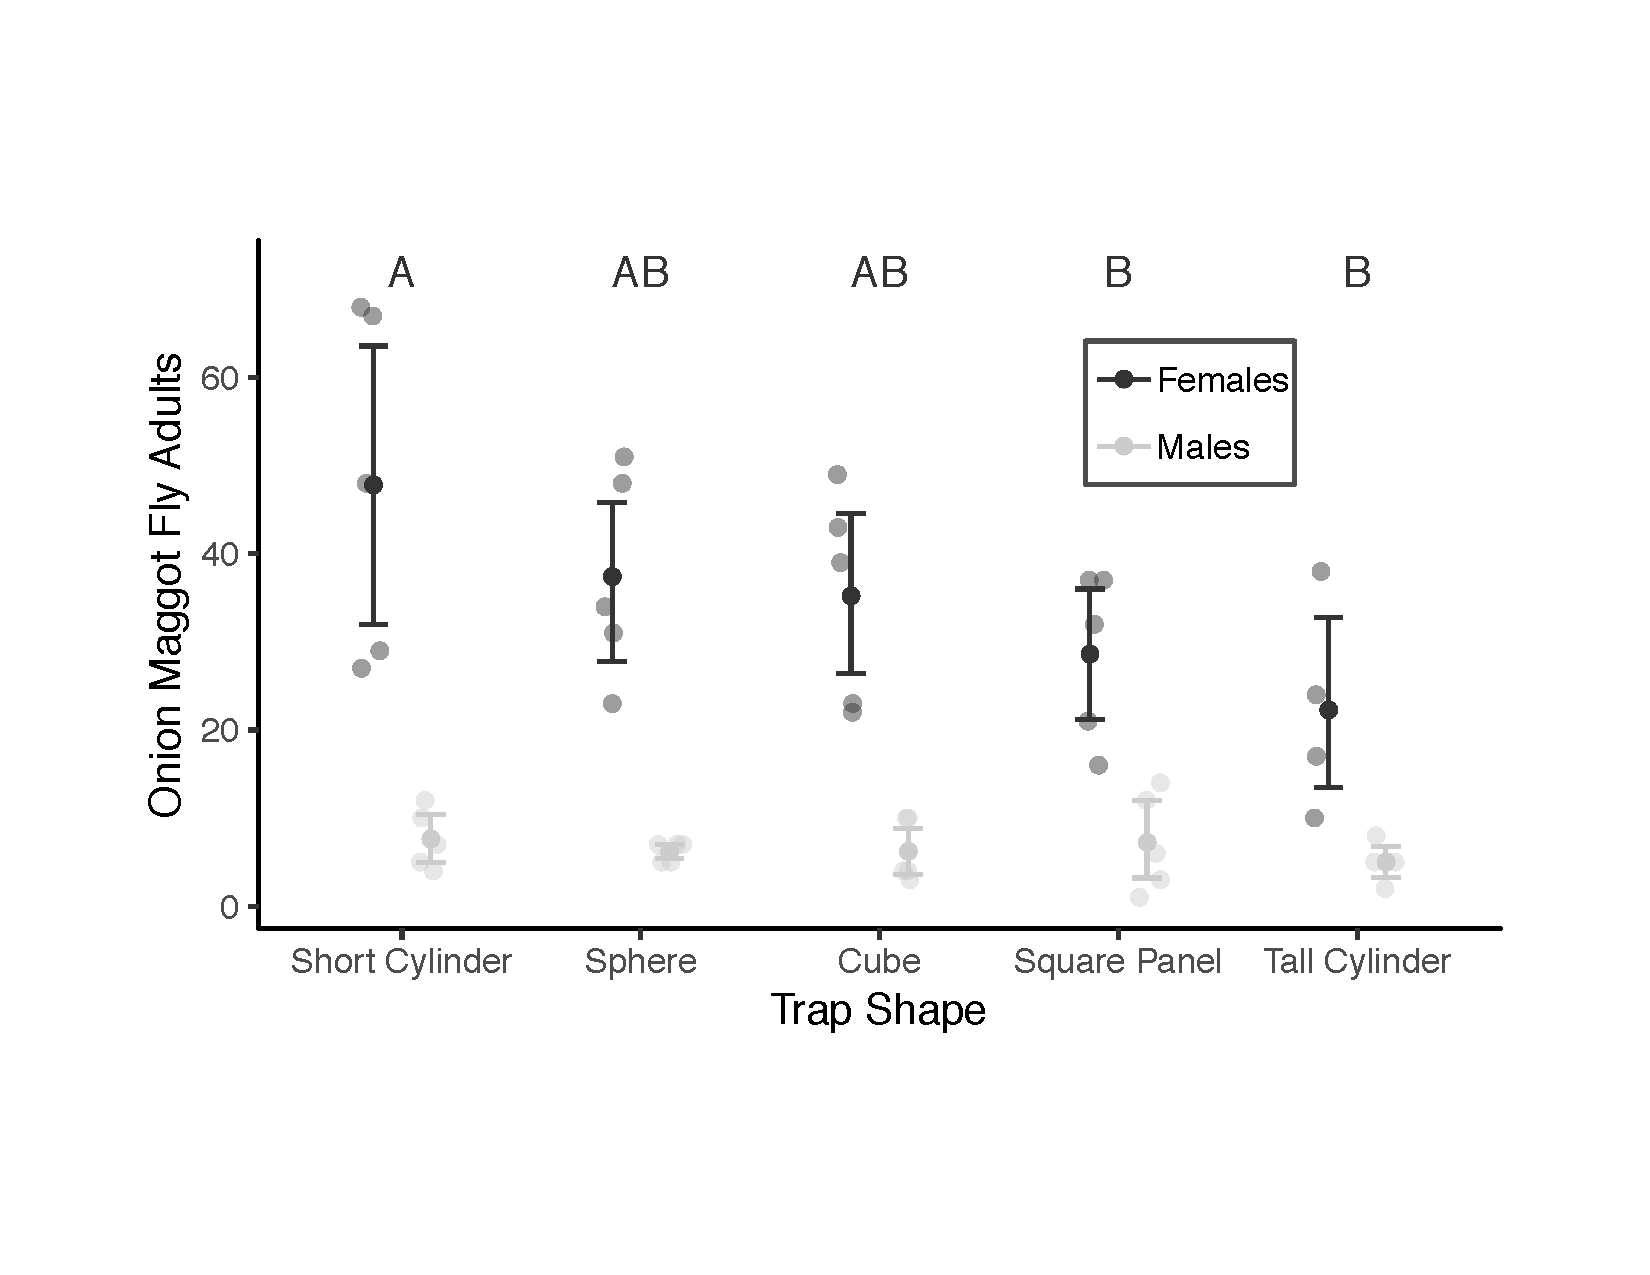
\includegraphics[width = 8cm]{figures/publication/figure-1.pdf}
\caption{\textit{D. antiqua} fly catch per trap over the sampling period on sticky traps of different shape.  Shaded points denote raw values while solid points and error bars denote mean and bootstrapped 95\% confidence intervals respectively.  Letters not shared between groups denote significant differences in female trap catch (there was no observed difference in male trap catch) at $\alpha$ = 0.05 with Tukey's HSD test. }
\label{fig:figure1}
\end{figure}

\begin{figure}[bt]
\centering
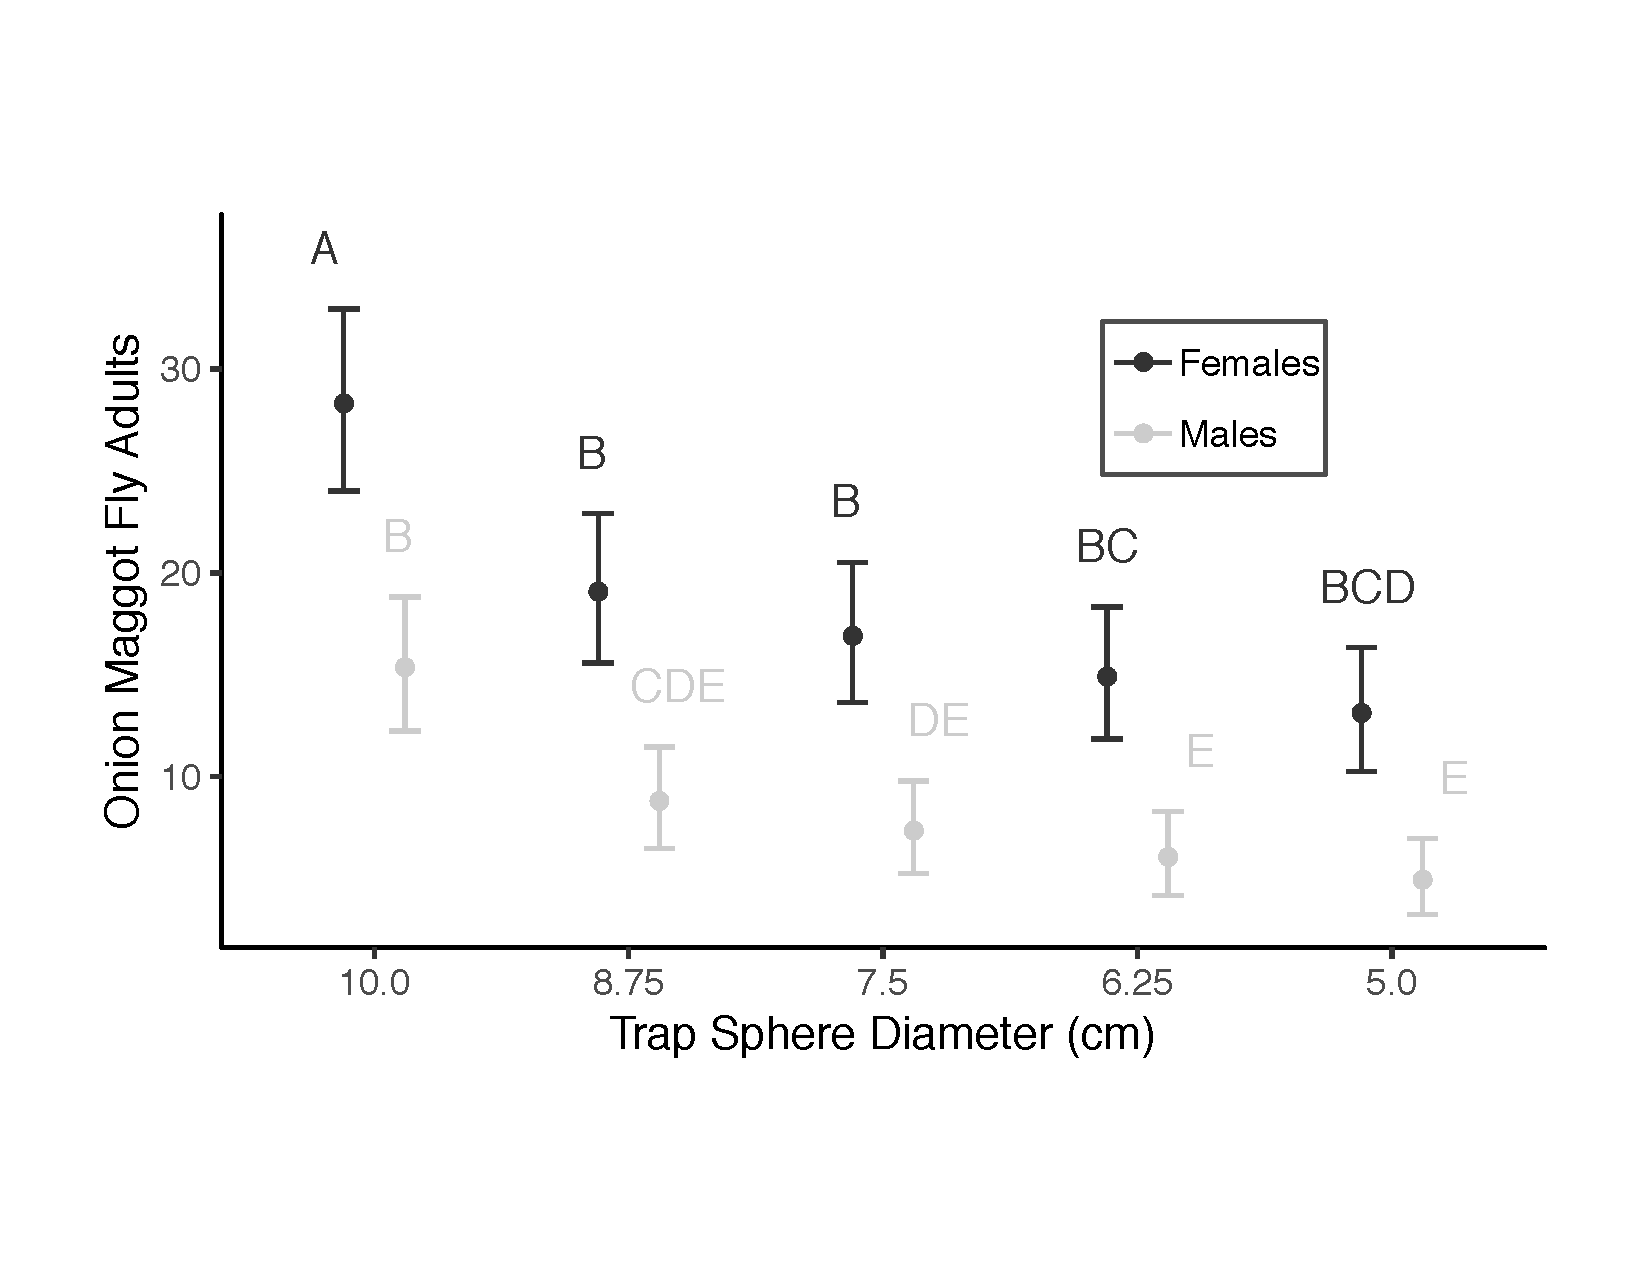
\includegraphics[width = 8cm]{figures/publication/figure-2.pdf}
\caption{\textit{D. antiqua} fly catch per trap over the sampling period on spherical sticky traps of different size.  Points and error bars denote mean and 95\% confidence intervals respectively.  Letters not shared between groups indicates significant differences in adult catch at $\alpha$ = 0.05 with Tukey's HSD test.}
\label{fig:figure2}
\end{figure}

\begin{figure}[bt]
\centering
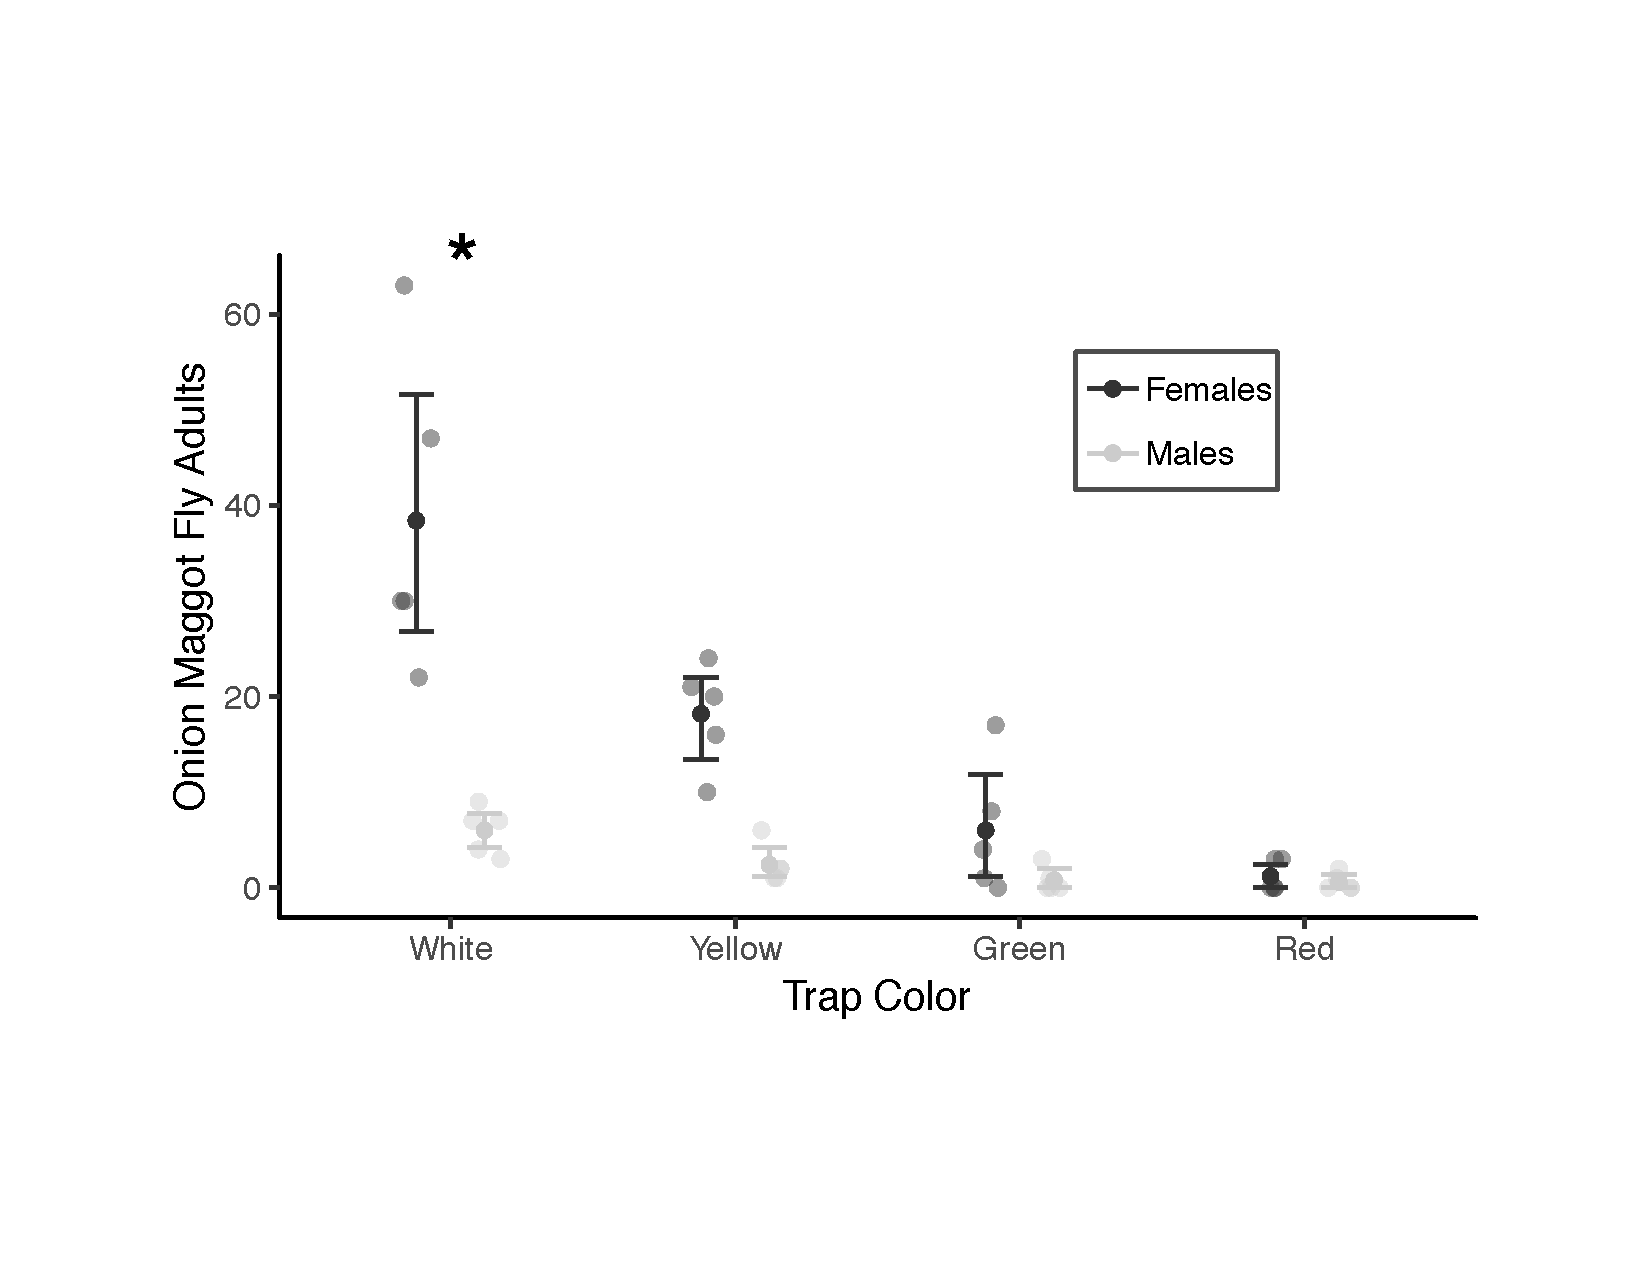
\includegraphics[width = 8cm]{figures/publication/figure-3.pdf}
\caption{\textit{D. antiqua} fly catch per trap over the sampling period on spherical sticky traps of different color.  Shaded points denote raw values while solid points and error bars denote means and bootstrapped 95\% confidence intervals respectively.  \textbf{*} indicates significantly different trap catch on white sticky traps (P = 0.012).}
\label{fig:figure3}
\end{figure}


\begin{figure}[bt]
\centering
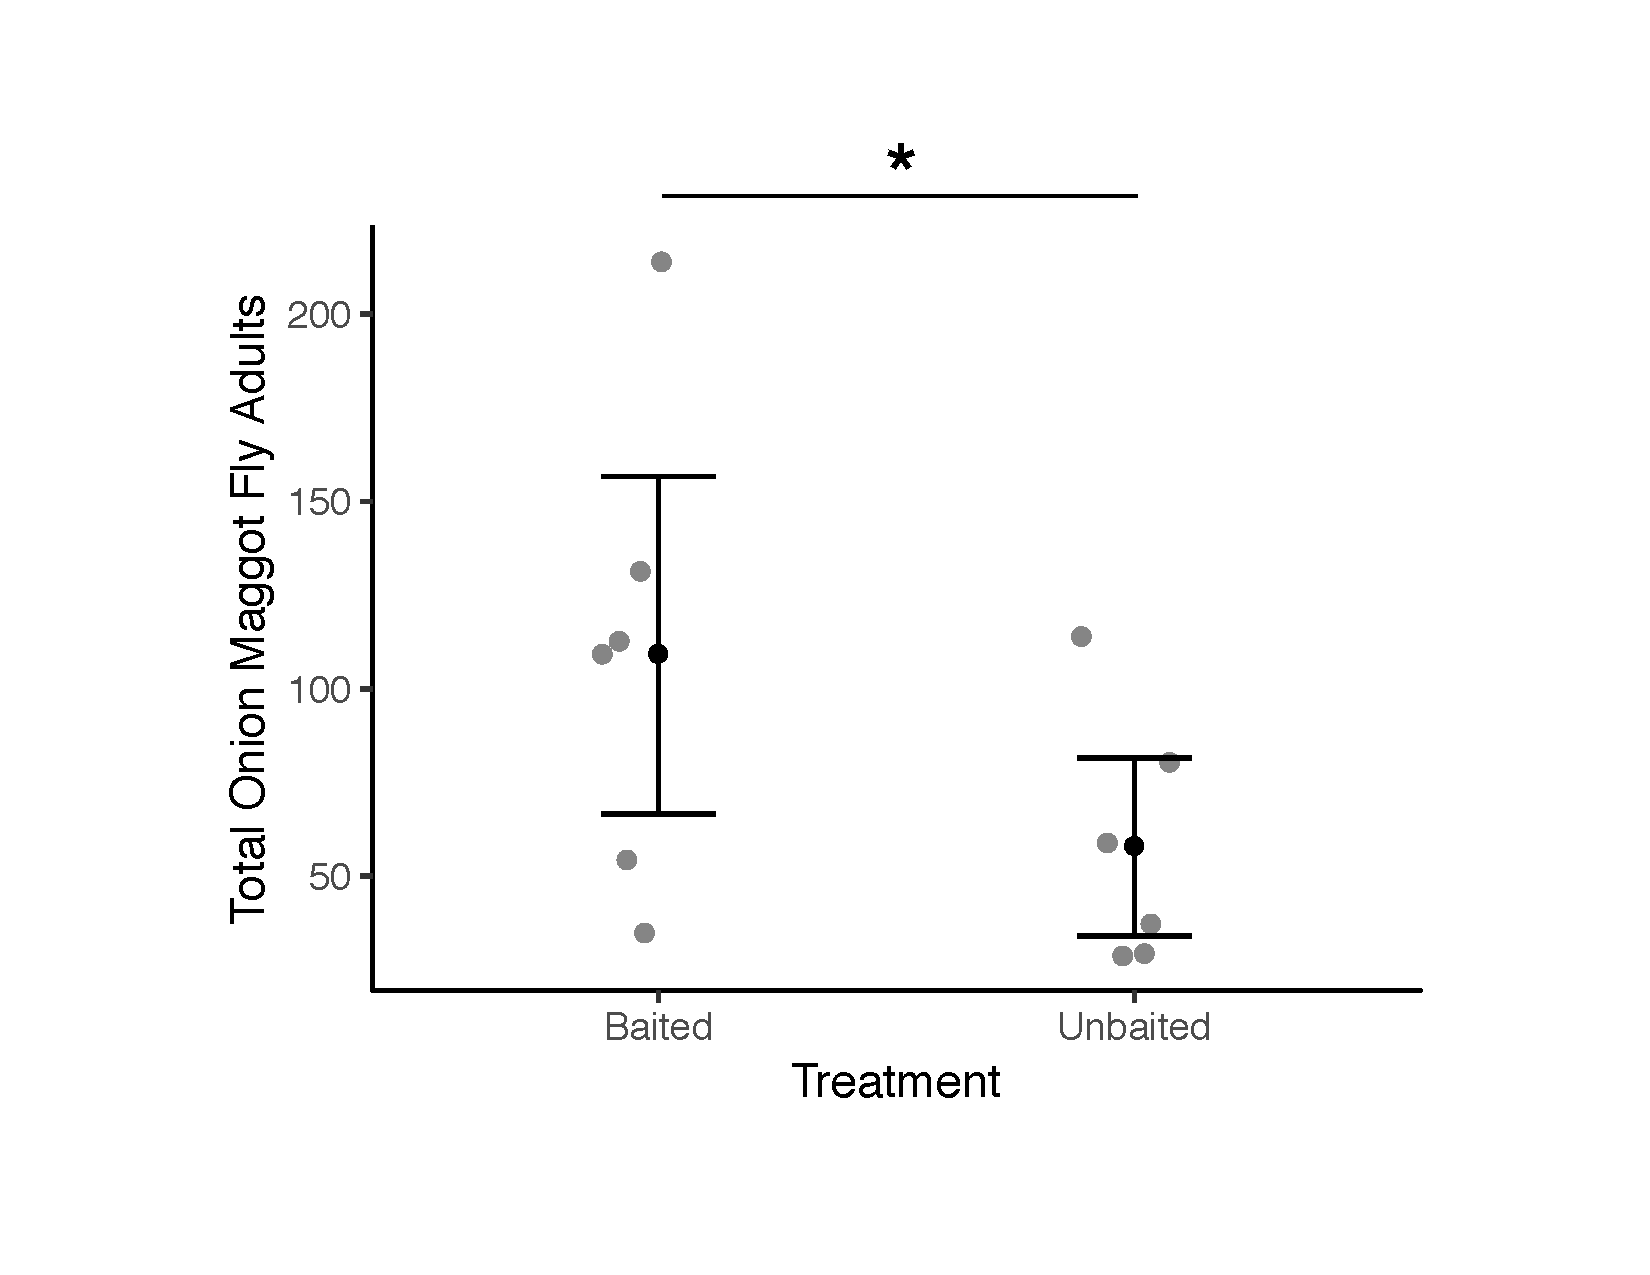
\includegraphics[width = 8cm]{figures/publication/figure-4.pdf}
\caption{\textit{D. antiqua} fly catch per trap over the sampling period on sticky traps baited with Delia Lure attractant and unbaited.  Shaded points denote raw values while solid points and error bars denote means and bootstrapped 95\% confidence intervals respectively.  \textbf{*} indicates significantly different trap catch on baited and unbaited traps (P = 0.030). }
\label{fig:figure4}
\end{figure}


\section{Discussion}

Varying the shape, size and color of sticky traps revealed that changes in these factors can increase catch of \textit{D. antiqua} flies.  Short cylinder traps performed better than most other shapes, but were not significantly different from spherical traps.  Spherical traps were more economical to produce and use so they were selected for use in subsequent studies.  Size played a large role in increasing trap catch.  Larger diameter traps with more surface area captured more adult \textit{D. antiqua} flies.  Color had perhaps the largest impact on catch of adult \textit{D. antiqua} flies with white traps far outperforming yellow, green and red traps.  

The combination of sticky traps with the chemical attractant, Delia Lure, also increased catch of adult \textit{D. antiqua} flies suggesting that \textit{D. antiqua} adults use a combination of visual and olfactory cues as suggested in previous studies \citep{harris1983color, harris1988host}.  Our work suggests that all of these factors play a role in \textit{D. antiqua} attraction in the field and expands upon previous work in the laboratory suggesting that no one factor is critical in \textit{D. antiqua} attraction \citep{harris1988host}.  

Sticky traps were chosen for this study in lieu of water traps because of their ease of use (replacing water is not necessary, and rain is not a problem) and because previous work has shown them to be more effective that water pan traps at catching \textit{D. antiqua} adults \citep{thomingdeveloping}.  This work showed that white traps far outperform sticky traps of other colors confirming findings in another study that white traps work well for \textit{Delia} flies.  Interestingly, other work has suggested that specificity for \textit{D. antiqua} could be improved with the color blue, but that overall trap catch may suffer \citep{thomingdeveloping}.   

These results suggest a way forward in improving trapping of \textit{D. antiqua} fly adults in the field. A spherical, white, large diameter sticky trap baited with Delia Lure is the best option for monitoring adult \textit{D. antiqua} flies based on the various factors tested in these trials. Improved trapping ability of white large diameter traps may improve monitoring efforts in situations where it is desirable to understand \textit{D. antiqua} phenology, develop decision support tools, measure range, and understand inter- and intra-generational spatio-temporal dynamics.  This improved trapping could then inform modeling efforts and predictive management abilities \citep{ning2017predicting, otto2000development,thomingdeveloping}.    

Sticky traps have been used in monitoring and control efforts of other visually responsive flies.  Orange spheres have been effective at attracting and trapping Caribbean Fruit Fly (\textit{Anastrepha suspensa} Lowe) \citep{sivinski1990colored}.  Apple maggot (\textit{Rhagoletis pomonella} Walsh) management, in particular, has benefited from development of red spherical traps for monitoring field populations \citep{prokopy1975apple, drummond1984comparative, duan1994apple}.  This work has even expanded into a control method by trapping apple maggot flies using these spheres in conjunction with other strategies, which hasreduced infestations \citep{bostanian1999managing}.  

The ability to attract larger numbers of adult \textit{D. antiqua} flies also creates an opportunity for a different, more environmentally friendly, management method. If larger numbers of flies can be attracted and then killed either by adhering to a sticky substance or coming into contact with an insecticide, populations of \textit{D. antiqua} could be reduced.  'Attract and kill' and 'Lure and kill' methodologies have been applied in pest management systems to moths, weevils, and other flies \citep{el2009potential,el2011bait,navarro2013efficacy,charmillot2000attract}.  Using large, white, spherical traps in conjunction with Delia Lure may provide the attraction needed to make it possible to control these pests using attract and kill strategies.  



\section*{Acknowledgements}
We appreciate technical assistance by M. Hessney and Delia Lure from J. Meneley. Starker Wright aided in the development and construction of traps as well as experimental design. The New York State Integrated Pest Management Program, USDA/CSREES Pest Management Alternatives Program, and New York State Department of Agriculture and Markets Onion Research and Development Program supported this research.  

\section*{Conflict of Interest}
The authors declare no conflict of interest.  

\section*{Author Contribution}
BAN and JPN conceived and conducted the experiments. DSW and CCF performed statistical analysis.  DSW, CCF, and BAN wrote the manuscript.  All authors read and approved the manuscript.    


\section*{Data Availability Statement}
All code and data, including manuscript documentation, is available on GitHub(https://github.com/acetworld/onion-maggot-attraction).

%\printendnotes

% Submissions are not required to reflect the precise reference formatting of the journal (use of italics, bold etc.), however it is important that all key elements of each reference are included.

\section{References}

\bibliographystyle{vancouver-authoryear}
\bibliography{om-attraction}

%\graphicalabstract{example-image-1x1}{Please check the journal's author guildines for whether a graphical abstract, key points, new findings, or other items are required for display in the Table of Contents.}

\end{document}
